\documentclass[12pt]{beamer}
\usetheme{Boadilla}
\usepackage{booktabs}
\usepackage{enumitem}
\usepackage{tikz}
\usepackage{pgfplots}
\usefonttheme{professionalfonts}
\renewcommand{\arraystretch}{1.25}
\usetikzlibrary{trees}
\title[ECON2843]{Lecture 5}
\subtitle{Part 2 Probability and Distributions}
\date{}
\usepackage{amsmath,amssymb,mathtools,wasysym}
\begin{document}
	\begin{frame}
		\titlepage
	\end{frame}
\begin{frame}{Marginal Probability}
	\begin{center}
		\begin{tabular}{lccc}
			\toprule
			&\parbox[t]{3cm}{$B_1$: Fund \\outperforms} &\parbox[t]{3cm}{$B_2$: Fund doesn't\\ outperform}&Totals\\
			\hline
			$A_1$: Rank $\le10$&0.06&0.16&0.22\\
			$A_2$: $10<$ Rank $<20$&0.05&0.13&0.18\\
			$A_3$: Rank $\ge20$&0.06&0.54&0.60\\
			\hline
			Totals&0.17&0.83&1\\
			\bottomrule
		\end{tabular}
	\end{center}
	For example:
	\begin{align*}
		P(A_1)&=P(A_1\cap B_1)+P(A_1\cap B_2)\\
		&=0.06+0.16\\
		&=0.22
	\end{align*}
\end{frame}
\begin{frame}{Law of Total Probability}
	
\begin{itemize}
\item[\color{blue}$\blacktriangleright$] What about $B_1$ (and $B_2$)? For example, why is the following true?
$$P(B_1)=P(B_1\cap A_1)+P(B_1\cap A_2)+P(B_1\cap A_3)$$
\item[\color{blue}$\blacktriangleright$] The previous result can be extended to apply to more than just an event and its complement.
\item[\color{blue}$\blacktriangleright$] More generally, it is called the {\bf Law of Total Probability}.
\end{itemize}
\end{frame}
\begin{frame}{Law of Total Probability}
	\begin{itemize}
		\item[\color{blue}$\blacktriangleright$] Suppose that the events $B_1, B_2, B_3,..., B_n$ are a partition/outcome of the sample space. That is:
		\begin{enumerate}[label=\textcolor{blue}{\arabic*.}]
			\item $B_1, B_2, B_3,..., B_n$ are mutually exclusive.
			\item $B_1\cup B_2\cup B_3\cup...\cup B_n=S$.
		\end{enumerate}
		\item[\color{blue}$\blacktriangleright$] Then for any event $A$, the following is true:
		$$P(A)=\sum_{i=1}^nP(A\cap B_i)$$
	\end{itemize}
\end{frame}
\begin{frame}{Law of Total Probability}
	\centering
	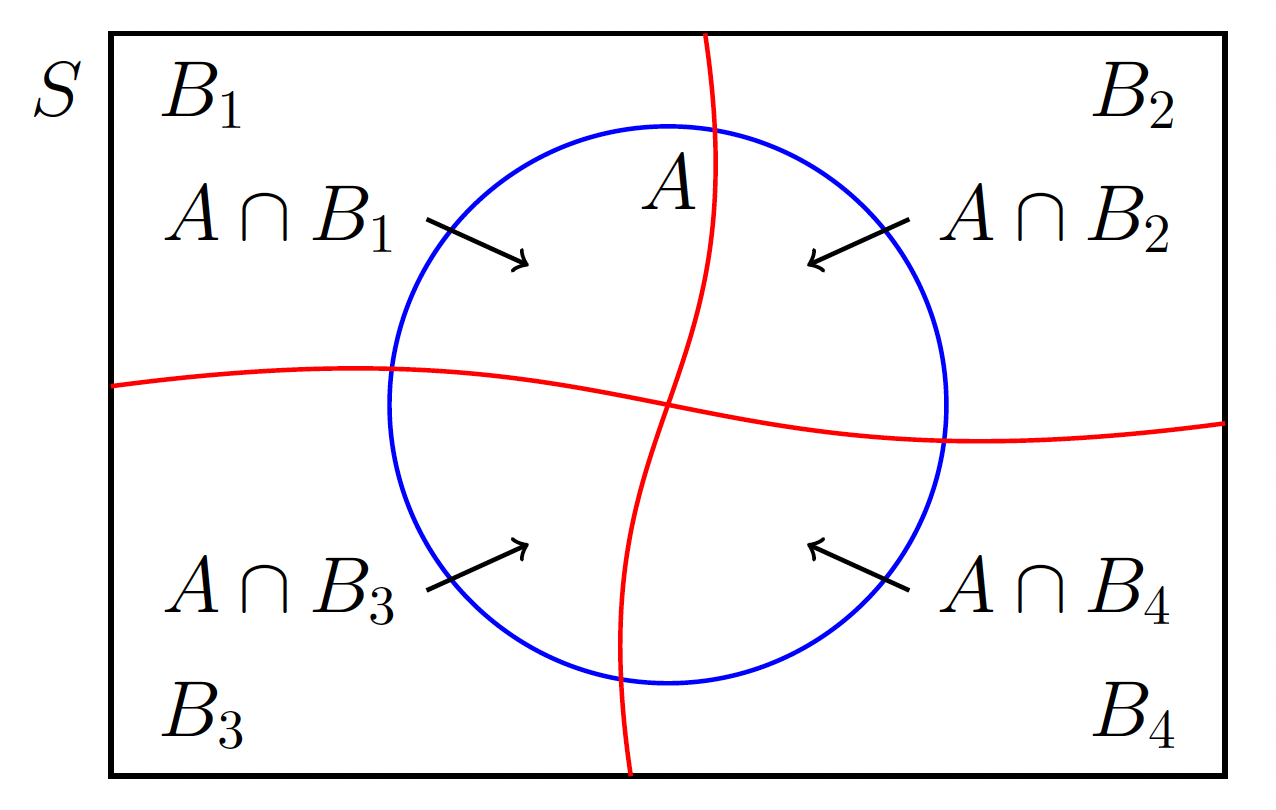
\includegraphics[width=8cm]{total.png}
\end{frame}
\begin{frame}{Conditional Probability}
\begin{itemize}
\item[\color{blue}$\blacktriangleright$] A conditional probability is the probability of one event, given the occurrence of another event.
\item[\color{blue}$\blacktriangleright$] For two events $A$ and $B$, the conditional probability of A given that B has occurred, denoted by $P(A|B)$, is defined to be:
$$P(A|B)=\frac{P(A\cap B)}{P(B)}$$
\end{itemize}
\end{frame}
\begin{frame}{Example}
	\begin{center}
		\begin{tabular}{lccc}
			\toprule
			&\parbox[t]{3cm}{$B_1$: Fund \\outperforms} &\parbox[t]{3cm}{$B_2$: Fund doesn't\\ outperform}&Totals\\
			\hline
			$A_1$: Rank $\le10$&0.06&0.16&0.22\\
			$A_2$: $10<$ Rank $<20$&0.05&0.13&0.18\\
			$A_3$: Rank $\ge20$&0.06&0.54&0.60\\
			\hline
			Totals&0.17&0.83&1\\
			\bottomrule
		\end{tabular}
	\end{center}
What is the probability that a fund with a manager from a top 10 program outperforms the market?
$$P(B_1|A_1)=\frac{P(B_1\cap A_1)}{P(A_1)}=\frac{0.06}{0.22}=0.2727$$
\end{frame}
\begin{frame}{Example}
	\begin{center}
		\begin{tabular}{lccc}
			\toprule
			&\parbox[t]{3cm}{$B_1$: Fund \\outperforms} &\parbox[t]{3cm}{$B_2$: Fund doesn't\\ outperform}&Totals\\
			\hline
			$A_1$: Rank $\le10$&0.06&0.16&0.22\\
			$A_2$: $10<$ Rank $<20$&0.05&0.13&0.18\\
			$A_3$: Rank $\ge20$&0.06&0.54&0.60\\
			\hline
			Totals&0.17&0.83&1\\
			\bottomrule
		\end{tabular}
	\end{center}
	For a fund that does not outperform the market,what is the probability that it was managed by someone from a top 10 program?
	$$P(A_1|B_2)=\frac{P(A_1\cap B_2)}{P(B_2)}=\frac{0.16}{0.83}=0.1928$$
\end{frame}
\begin{frame}{Independence}
\begin{itemize}
	\item[\color{blue}$\blacktriangleright$] Two events $A$ and $B$ are independent if and only if the following holds:
	$$P(A\cap B)=P(A)\times P(B)$$
	\item[\color{blue}$\blacktriangleright$] We can derive a more intuitive definition of independence by looking at what happens to the conditional probabilities $P(A|B)$ and $P(B|A)$.
\end{itemize}
\end{frame}
\begin{frame}{Independence}
	\begin{itemize}
		\item[\color{blue}$\blacktriangleright$] If $A$ and $B$ are independent:
		$$P(A|B)=\frac{P(A\cap B)}{P(B)}=\frac{P(A)\times P(B)}{P(B)}=P(A)$$
		$$P(B|A)=\frac{P(B\cap A)}{P(A)}=\frac{P(B)\times P(A)}{P(A)}=P(B)$$
		\item[\color{blue}$\blacktriangleright$] That is, two events are independent if the probability of one event occurring is not affected by the occurrence of the other event.
	\end{itemize}
\end{frame}
\begin{frame}{Example}
	\begin{itemize}
		\item[\color{blue}$\blacktriangleright$] If $A$ and $B$ are independent:
		$$P(A|B)=\frac{P(A\cap B)}{P(B)}=\frac{P(A)\times P(B)}{P(B)}=P(A)$$
		$$P(B|A)=\frac{P(B\cap A)}{P(A)}=\frac{P(B)\times P(A)}{P(A)}=P(B)$$
		\item[\color{blue}$\blacktriangleright$] That is, two events are independent if the probability of one event occurring is not affected by the occurrence of the other event.
	\end{itemize}
\end{frame}
\begin{frame}{Example}
	\begin{itemize}
		\item[\color{blue}$\blacktriangleright$] A store sells two brands of a particular product, one expensive ($A$) and the other inexpensive ($B$).
		\item[\color{blue}$\blacktriangleright$] A survey of 1000 sales gave the following results:
	\begin{center}
		\begin{tabular}{cccc}
			\toprule
			&$A$&$B$&Totals\\
			\hline
			Male&132&147&279\\
			Female&516&205&721\\
			\hline
			Totals&648&352&1000\\
			\bottomrule
		\end{tabular}
	\end{center}
	\item[\color{blue}$\blacktriangleright$] Are the events "being female" and "purchasing brand $A$" independent?
	\end{itemize}
\end{frame}
\begin{frame}{Example}
		\begin{center}
			\begin{tabular}{cccc}
				\toprule
				&$A$&$B$&Totals\\
				\hline
				Male&132&147&279\\
				Female&516&205&721\\
				\hline
				Totals&648&352&1000\\
				\bottomrule
			\end{tabular}
		\end{center}
		$$P(A\cap \text{Female})=\frac{516}{1000}=0.516$$
		$$P(A)\times P(\text{Female})=\frac{648}{1000}\times\frac{721}{1000}=0.467208$$
	\begin{itemize}
		\item[\color{blue}$\blacktriangleright$] Not independent since
		$$P(A\cap \text{Female})\ne P(A)\times P(\text{Female}).$$
	\end{itemize}
\end{frame}
\begin{frame}{Multiplication Rule}
	\begin{itemize}
		\item[\color{blue}$\blacktriangleright$] For two events $A$ and $B$, the {\bf Multiplication Rule} states:
		$$P(A\cap B)=P(A|B)\times P(B)=P(B|A)\times P(A)$$
		\item[\color{blue}$\blacktriangleright$] The rule follows directly from the definition of conditional probability.
		\item[\color{blue}$\blacktriangleright$] Note that if $A$ and $B$ are independent, the multiplication rule gives us:
		$$P(A\cap B)=P(A)\times P(B)$$
	\end{itemize}
\end{frame}
\begin{frame}{Example}
	\begin{itemize}
		\item[\color{blue}$\blacktriangleright$] A finance course has 15 male and 10 female students. Each week, the lecturer wants to select two different students at random to ask questions during class. What is the probability that the two students chosen are female?
		\item[\color{blue}$\blacktriangleright$] Let's define some events:
		\begin{itemize}
			\item Let $A$ be the event that the first student chosen is female.
			\item Let $B$ be the event that the second student chosen is female.
		\end{itemize}
		\item[\color{blue}$\blacktriangleright$] We want to find $P(A\cap B)$.
	\end{itemize}
\end{frame}
\begin{frame}{Example}
	\begin{itemize}
		\item[\color{blue}$\blacktriangleright$] Using the Multiplication Rule:
		$$P(A\cap B)=P(B|A)\times P(A)$$
		\item[\color{blue}$\blacktriangleright$] We know:
		$$P(A)=\frac{10}{25}\text{   and   }P(B|A)=\frac{9}{24}$$
		\item[\color{blue}$\blacktriangleright$] Therefore
		$$P(A\cap B)=\frac{10}{25}\times\frac{9}{24}=0.15$$
	\end{itemize}
\end{frame}
\begin{frame}{Example}
	\begin{itemize}
		\item[\color{blue}$\blacktriangleright$] If the lecturer decides to select three students instead of two, what is the probability that the first student chosen is female and the next two are male?
		\item[\color{blue}$\blacktriangleright$] Again we define some events:
		\begin{itemize}
			\item Let $A$ be the event that the first student chosen is female.
			\item Let $B$ be the event that the second student chosen is male.
			\item Let $C$ be the event that the third student chosen is male.
		\end{itemize}
		\item[\color{blue}$\blacktriangleright$] We want to find $P(A\cap B\cap C)$.
	\end{itemize}
\end{frame}
\begin{frame}{Example}
	\begin{itemize}
		\item[\color{blue}$\blacktriangleright$] Using the multiplication rule:
		\begin{align*}
		P(A\cap B\cap C)&=P(C|(A\cap B))\times P(A\cap B)\\
		&=P(C|(A\cap B))\times P(B|A)\times P(A)
	\end{align*}
		
		\item[\color{blue}$\blacktriangleright$] We know:
		$$P(A)=\frac{10}{25},\quad P(B|A)=\frac{15}{24},\quad P(C|(A\cap B)=\frac{14}{23}$$
		\item[\color{blue}$\blacktriangleright$] Therefore
		$$P(A\cap B\cap C)=\frac{10}{25}\times\frac{15}{24}\times\frac{14}{23}=0.1522$$
	\end{itemize}
\end{frame}
\begin{frame}{Addition Rule}
	\begin{itemize}
		\item[\color{blue}$\blacktriangleright$] For two events $A$ and $B$, the {\bf Addition Rule} states:
		$$P(A\cup B)=P(A)+P(B)-P(A\cap B)$$
		
		\item[\color{blue}$\blacktriangleright$] Why do we need to subtract $P(A\cap B)$
	\end{itemize}
		\centering
	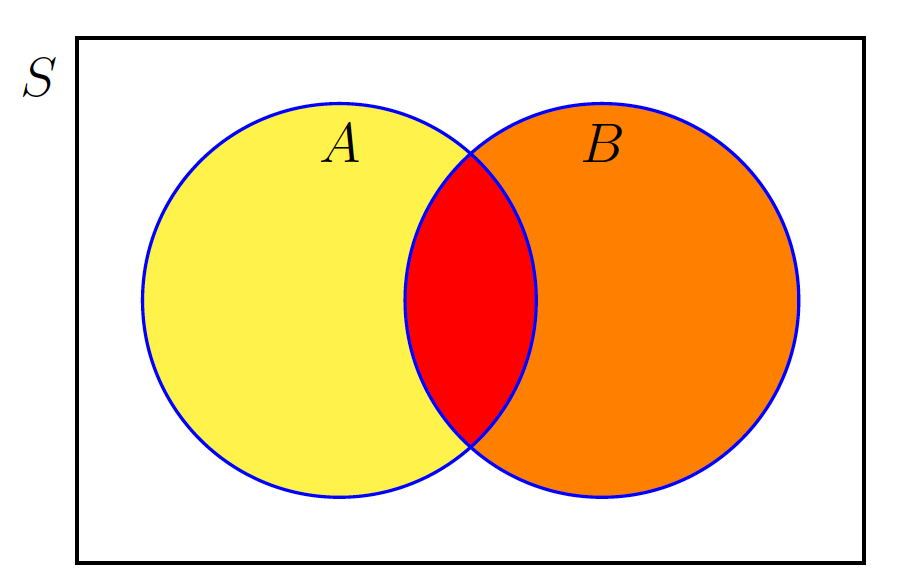
\includegraphics[width=8cm]{addition.png}
\end{frame}
\begin{frame}{Addition Rule}
	\begin{itemize}
		\item[\color{blue}$\blacktriangleright$] If $A$ and $B$ are mutually exclusive, the Addition Rule reduces to:
		$$P(A\cup B)=P(A)+P(B)$$
	\end{itemize}
	\centering
	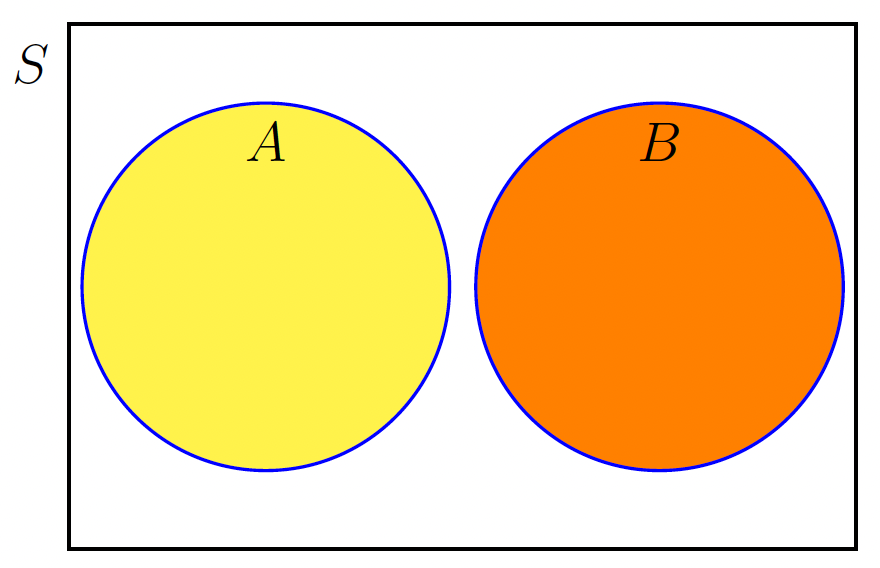
\includegraphics[width=8cm]{reduce.png}
\end{frame}
\begin{frame}{Complement Rule}
	\begin{itemize}
		\item[\color{blue}$\blacktriangleright$] For an event $A$, the Complement Rule states:
		\item[\color{blue}$\blacktriangleright$] Proof:
		\begin{align*}
			A^C\cup A&=S\\
			P(A^C\cup A)&=P(S)\\
			\text{applying addition rule: }P(A^C)+P(A)&=1\\
			P(A^C)&=1-P(A)
		\end{align*}
	\end{itemize}
\end{frame}
\begin{frame}{Example}
	\begin{itemize}
		\item[\color{blue}$\blacktriangleright$] Suppose we flip a fair coin eight times. (How many outcomes do we have?)
		\item[\color{blue}$\blacktriangleright$] Find the probability of getting at least one tail.
		\item[\color{blue}$\blacktriangleright$] Let $A$ be the event "at least one tail".
				\begin{align*}
			A=\{&THHHHHHH,HTHHHHHH,\cdots\\
			&TTHHHHHH,HTTHHHHH,\cdots\\
			&\cdots\}
		\end{align*}
	\end{itemize}
\end{frame}
\begin{frame}{Example}
	\begin{itemize}
		\item[\color{blue}$\blacktriangleright$] Using the Complement Rule:
			\end{itemize}
		\begin{align*}
			P(A)&=1-P(A^C)\\
			&=1-P(\text{flipping no tails})\\
			&=1-P(\text{flipping eight heads})\\
			&=1-(\frac{1}{2})^8\\
			&=\frac{255}{256}=0.9961
		\end{align*}

\end{frame}
\begin{frame}{Example 1}
	\begin{itemize}
		\item[\color{blue}$\blacktriangleright$] Bad gums may mean a bad heart. Researchers discovered that 85\% of people who have suffered a heart attack had periodontal disease. Only 29\% of healthy people have this disease. Suppose that in a certain community heart attacks occur with 10\% probability. If someone had periodontal disease,what is the probability that he or she will have a heart attack?
	\end{itemize}
	
\end{frame}
\begin{frame}{Solution}
	\begin{itemize}
		\item[\color{blue}$\blacktriangleright$] Let $D$ be the event "have periodontal disease".
		\item[\color{blue}$\blacktriangleright$] Let $H$ be the event "have suffered a heart attack".
		\item[\color{blue}$\blacktriangleright$] What we know:
		\begin{itemize}
			\item $P(H)=0.1$, so therefore $P(H^C)=0.9$.
			\item $P(D|H)=0.85$.
			\item $P(D|H^C)=0.29$.
		\end{itemize}
		\item[\color{blue}$\blacktriangleright$] We want to find $P(H|D)$.
	\end{itemize}
	
\end{frame}
\begin{frame}{Solution}
	\begin{itemize}
		\item[\color{blue}$\blacktriangleright$] From the definition of conditional probability:
		$$P(H|D)=\frac{P(H\cap D)}{P(D)}$$
		\item[\color{blue}$\blacktriangleright$] For the numerator, we can use the Multiplication Rule:
	\end{itemize}
	\begin{align*}
		P(H\cap D)&=P(D|H)\times P(H)\\
		&=0.85\times0.1\\
		&=0.085
	\end{align*}
	
\end{frame}

\begin{frame}{Solution}
	\begin{itemize}
		\item[\color{blue}$\blacktriangleright$] For the denominator, we can use the Law of Total Probability:
		$$P(D)=P(D\cap H)+P(D\cap H^C)$$
		\item[\color{blue}$\blacktriangleright$] For the second term above, we again use the Multiplication Rule:
	\end{itemize}
	\begin{align*}
		P(D\cap H^C)&=P(D|H^C)\times P(H^C)\\
		&=0.29\times0.9\\
		&=0.261
	\end{align*}
	
\end{frame}

\begin{frame}{Solution}
	\begin{itemize}
		\item[\color{blue}$\blacktriangleright$] Therefore we get:
		$$P(D)=0.085+0.261=0.346$$
		\item[\color{blue}$\blacktriangleright$] Putting the numerator and denominator together, we get:
	\end{itemize}
	\begin{align*}
		P(H|D)&=\frac{P(H\cap D)}{P(D)}\\
		&=\frac{0.085}{0.346}\\
		&=0.2457
	\end{align*}
	
\end{frame}
\begin{frame}{Example 2}
	\begin{itemize}
		\item[\color{blue}$\blacktriangleright$] A construction company has bid on two contracts. The probability of winning contract $A$ is 0.3. If the company wins contract $A$, then the probability of winning contract $B$ is 0.4. If the company loses contract $A$, then the probability of winning contract $B$ decreases to 0.2.Find the probability of the following events:
	\end{itemize}
	\begin{enumerate}[label=\textcolor{blue}{(\alph*)}]
		\item Winning both contracts.
		\item Winning exactly one contract.
		\item Winning at least one contract.
	\end{enumerate}
	
\end{frame}

\begin{frame}{Solution}
	\begin{itemize}
		\item[\color{blue}$\blacktriangleright$] Let $A$ be the event "win contract $A$".
		\item[\color{blue}$\blacktriangleright$] Let $B$ be the event "win contract $B$".
		\item[\color{blue}$\blacktriangleright$] We know:
		\begin{itemize}
			\item $P(A)=0.3$.
			\item $P(B|A)=0.4$.
			\item $P(B|A^C)=0.2$.
		\end{itemize}
		\item[\color{blue}$\blacktriangleright$] Can be helpful to fill out a joint probability table.
	\end{itemize}
\end{frame}
\begin{frame}{Solution}
		\begin{center}
	\begin{tabular}{cccc}
		\toprule
		&$B$&$B^C$&Totals\\
		\hline
		$A$&$P(A\cap B)$&$P(A\cap B^C)$&$P(A)$\\
		$A^C$&$P(A^C\cap B)$&$P(A^C\cap B^C)$&$P(A^C)$\\
		\hline
		Totals&$P(B)$&$P(B^C)$&1\\
		\bottomrule
	\end{tabular}
\end{center}
\end{frame}
\begin{frame}{Solution}
	\begin{center}
		\begin{tabular}{cccc}
			\toprule
			&$B$&$B^C$&Totals\\
			\hline
			$A$&0.12&0.18&0.3\\
			$A^C$&0.14&0.56&0.7\\
			\hline
			Totals&0.26&0.74&1\\
			\bottomrule
		\end{tabular}
	\end{center}
	$$P(A\cap B)=P(B|A)\times P(A)=0.4\times0.3=0.12$$
	$$P(A^C\cap B)=P(B|A^C)\times P(A^C)=0.2\times0.7=0.14$$
\end{frame}
\begin{frame}{Solution}
	\begin{center}
		\begin{tabular}{cccc}
			\toprule
			&$B$&$B^C$&Totals\\
			\hline
			$A$&0.12&0.18&0.3\\
			$A^C$&0.14&0.56&0.7\\
			\hline
			Totals&0.26&0.74&1\\
			\bottomrule
		\end{tabular}
	\end{center}
	\begin{enumerate}[label=\textcolor{blue}{(\alph*)}]
	\item Winning both contracts: $P(A\cap B)=0.12$.
	\item Winning exactly one contract:
	$$P(A\cap B^C)+P(A^C\cap B)=0.18+0.14=0.32.$$
	\item Winning at least one contract:
	$$1-P(A^C\cap B^C)=1-0.56=0.44.$$
\end{enumerate}
\end{frame}

\begin{frame}{Example 3}
	\begin{itemize}
		\item[\color{blue}$\blacktriangleright$] Suppose we flip a fair 1 dollar coin four times and,independently, we flip a 50 cent coin three times.
	\end{itemize}
	\begin{enumerate}[label=\textcolor{blue}{(\alph*)}]
		\item Find the probability of flipping three tails on the 1 dollar coin or flipping two tails on the 50 cent coin.
		\item Given that the total number of tails across all flips of both coins is five, find the probability of flipping three tails on the 1 dollar coin.
	\end{enumerate}
	
\end{frame}
\begin{frame}{Solution - Part (a)}
	\begin{itemize}
	\item[\color{blue}$\blacktriangleright$] Let $A_3$ be the event "flipping three tails on the 1 dollar coin".
	$$A_3=\{TTTH,TTHT,THTT,HTTT\}$$
	Therefore,
	$$P(A_3)=\frac{4}{2^4}=\frac{1}{4}$$
	\item[\color{blue}$\blacktriangleright$] Let $B_2$ be the event "flipping two tails on the 50 cent coin".
	$$B_2=\{TTH,THT,HTT\}$$
	Therefore,
	$$P(B_2)=\frac{3}{2^3}=\frac{3}{8}$$
\end{itemize}
\end{frame}
\begin{frame}{Solution - Part (a)}
	\begin{itemize}
		\item[\color{blue}$\blacktriangleright$] We want to find $P(A3\cup B2)$. Using the Addition Rule together with the independence of $A_3$ and $B_2$:
			\end{itemize}
\begin{align*}
	P(A_3 \cup B_2) &= P(A_3) + P(B_2) - P(A_3 \cap B_2) \\
	&= P(A_3) + P(B_2) - P(A_3) \times P(B_2) \\
	&= \frac{1}{4} + \frac{3}{8} - \frac{1}{4} \times \frac{3}{8} \\
	&= \frac{17}{32} \\
	&= 0.5313
\end{align*}

\end{frame}
\begin{frame}{Solution - Part (b)}
\begin{itemize}
	\item[\color{blue}$\blacktriangleright$] Let $A_3$ be defined as before and let $C$ be the event "flipping five tails across all flips of both coins''.
	\item[\color{blue}$\blacktriangleright$] We want to find
	\[P(A_3|C) = \frac{P(A_3 \cap C)}{P(C)}\]
	\item[\color{blue}$\blacktriangleright$] Note that $A_3 \cap C = A_3 \cap B_2$.
	\item[\color{blue}$\blacktriangleright$] Therefore
	\[P(A_3 \cap C) = P(A_3) \times P(B_2) = \frac{1}{4} \times \frac{3}{8} = \frac{3}{32}\]
\end{itemize}
	
\end{frame}
\begin{frame}{Solution - Part (b)}
\begin{itemize}
	\item[\color{blue}$\blacktriangleright$] Also, $C = (A_2 \cap B_3) \cup (A_3 \cap B_2) \cup (A_4 \cap B_1)$, so:
	\begin{align*}
		P(C) &= P((A_2 \cap B_3) \cup (A_3 \cap B_2) \cup (A_4 \cap B_1)) \\
		&= P(A_2 \cap B_3) + P(A_3 \cap B_2) + P(A_4 \cap B_1) \\
		&= P(A_2) \times P(B_3) + P(A_3) \times P(B_2) \\
		&\quad + P(A_4) \times P(B_1) \\
		&= \frac{3}{8} \times \frac{1}{8} + \frac{1}{4} \times \frac{3}{8} + \frac{1}{16} \times \frac{3}{8} = 0.1641
	\end{align*}
	
	\item[\color{blue}$\blacktriangleright$] Therefore,
	\[P(A_3|C) = \frac{\frac{3}{32}}{0.1641} = 0.5714\]
\end{itemize}
\end{frame}
\begin{frame}{Example 4}
	\begin{itemize}
		\item[\color{blue}$\blacktriangleright$] There are three buckets that weigh 1lb, 2lb and3lb, respectively. A bucket weighing $i$ lb contains $i$ white balls and $5 - i$ black balls, for $i = 1,2,3$. For example, the bucket weighing 1lb contains 1 white ball and 4 black balls. Suppose a bucket is chosen with probability proportional to its weight and two balls are randomly selected (without replacement) from this bucket.
	\end{itemize}
	\begin{enumerate}[label=\textcolor{blue}{(\alph*)}]
		\item Find the probability that both balls selected are white.
		\item If both balls selected are white, what is the probability that the bucket weighing 3lb was chosen?
	\end{enumerate}
	
\end{frame}
\end{document}